\section{Glance Gitlab integration}
\label{sec:glance-gitlab-integration}

As already said before, the Glance Phase 0 originated from the need to have an automatic creation of Gitlab repositories for each Analysis or publication. So Phase 0 interface has some buttons that triggers the communication with Gitlab.

A basic structure is already set in Gitlab to store the groups related to an Analysis. The main Gitlab group is called atlas-physics-office and it stores many subgroups. Each of those subgroups belong to a leading group, for example: Higgs and Exotics.

\begin{figure}[ht!]
  \centering
  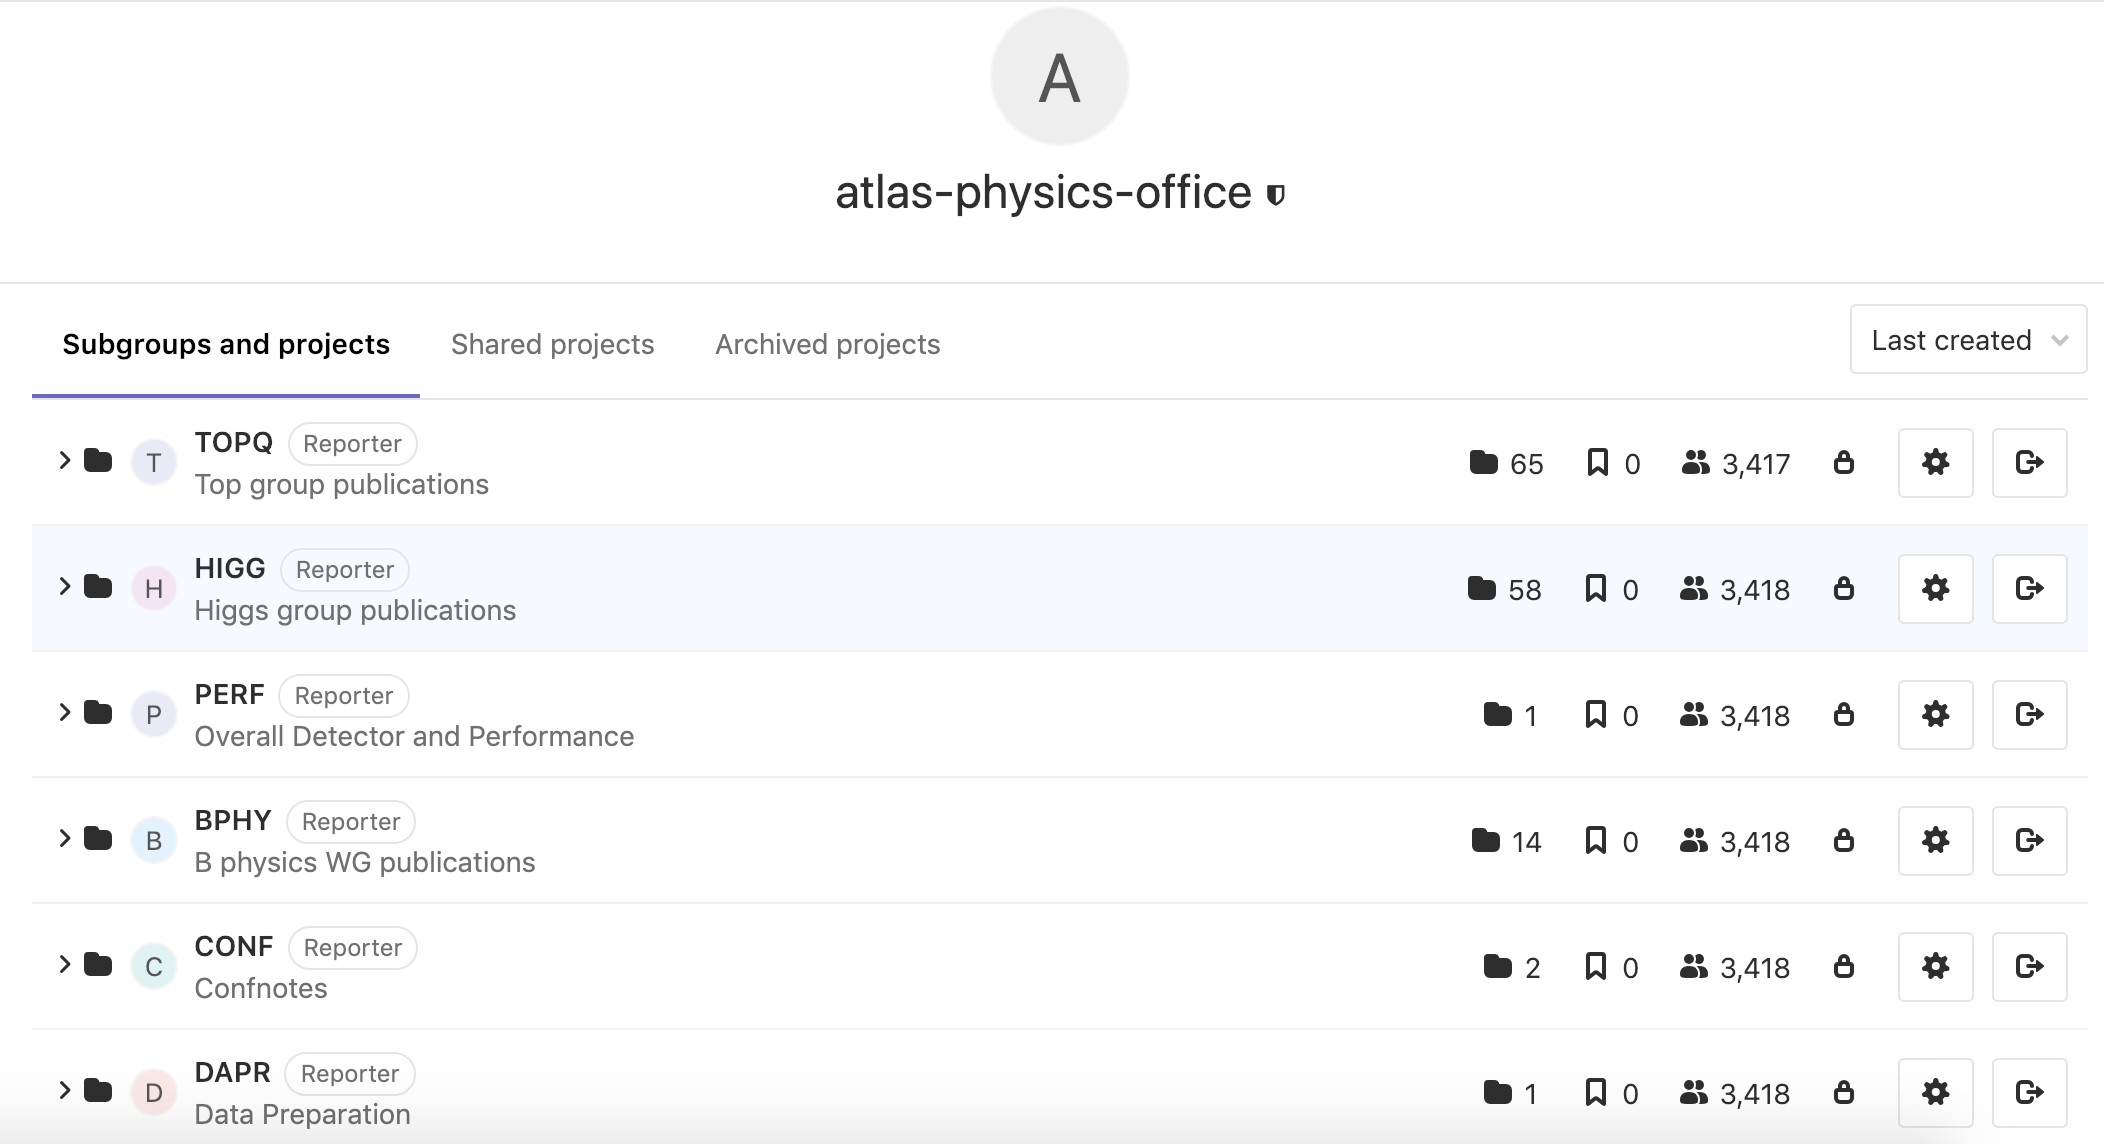
\includegraphics[width=0.9\textwidth]{po-lead-groups-tree.png}
  \caption{Screenshot of leading groups Gitlab infrastructure.}
  \label{fig:po-lead-groups-tree}
\end{figure}

When a Phase 0 entry is created through Glance, a group with its reference code is automatically created containing the first internal note repository. The content of this repository's first commit is get from a source repository with file templates called atlaslatex, also inside atlas-physics-office group. Glance is responsible to substitute the variables in all the file templates according to the metadata inserted when creating the entry in the system. After the commit, Glance automatically unprotects the master branch, creates the protected PO-ready branch and also created PO-Publication label. The last thing done in this first integration is to set the developer permission to the Analysis Team egroup.

Another Glance and Gitlab integration happens when Phase 0 finished or it is skipped, proceeding to Paper, CONF or PUB note Phase 1. When this happens, Glance automatically creates a configured repository inside the Analysis group belonging to the respective publication. It is also possible to add one or more additional internal note repositories at any time.

\begin{figure}[ht!]
  \centering
  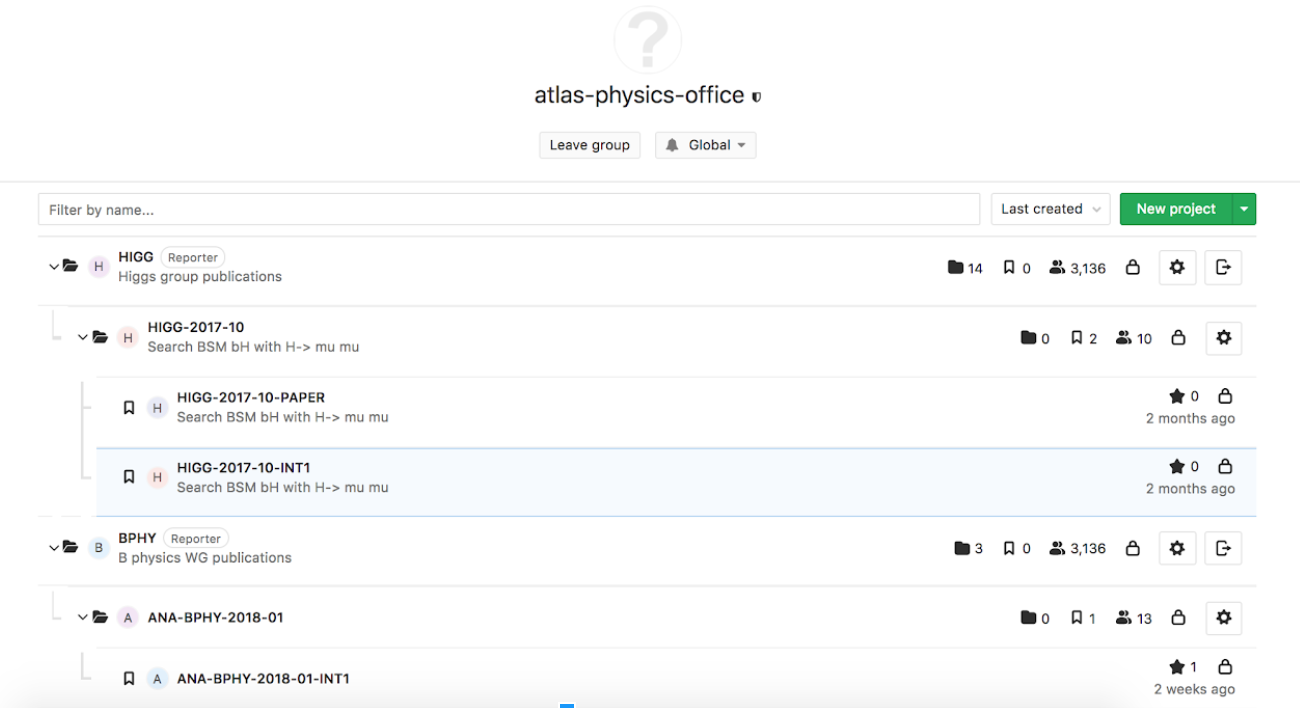
\includegraphics[width=0.9\textwidth]{po-ana-tree.png}
  \caption{Screenshot of Analysis Phase 0 groups Gitlab infrastructure.}
  \label{fig:po-ana-tree}
\end{figure}

\subsection{Authorlist and Acknowledgement}

Authorlists and Acknowledgements are two of the main steps of a paper’s publication and both are treated, ad generated, using the Fence system. 
The authorlist is the entire list of ATLAS’s authors (normal or exceptional) that take part to the creation of the publications, every paper have a different authorlist (the authorlist creation is based on the paper reference date) and it is build following restrictive rules and milestones.
The acknowledgement is the list of all the Founding agencies that support the ATLAS organisation on the publication process of each papers. This list change less often than the authorlist but it have anyway restrictive rules to follow.
Both of this list will be included into the final files that are send to the journal for the publication and will be printed out on the final release, that’s why ATLAS take care a lot about the creation and the maintenance of the two. 

\subsection{Fence Authorlist interfaces main functionalities (Gitlab, AFS ...)}

One interface has been created, https://glance.cern.ch/atlas/membership/authorlists, where a resumee of all the author lists can be found and easily filtered through the SEARCH option.
All the columns are self-explanatory; the last one gives access to the author list location, which can be distinguished by the icon: a download icon means the files are stored in AFS and can be downloaded on your local machine, a GitLab icon means the paper was produced through the Glance / GitLab integration and the files can be viewed directly on your browser. 

\begin{figure}[ht!]
  \centering
  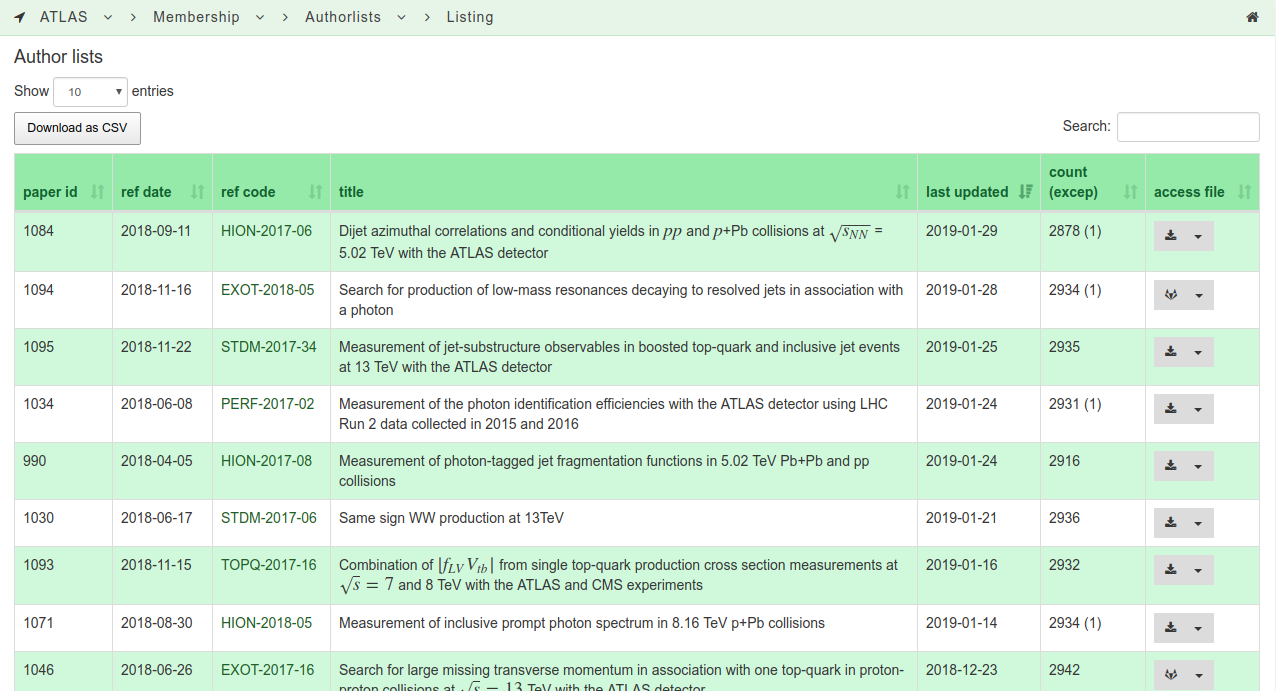
\includegraphics[width=0.9\textwidth]{authorlist.png}
  \caption{Screenshot of Fence Authorlist interface. The second one in the list is a GitLab project.}
  \label{fig:po-ana-tree}
\end{figure}

Another interface, https://glance.cern.ch/atlas/membership/authorlists/generate, is available to get a preview of the authorlist at the current date. Here a complete list of authors, institutes and footnotes for the authorlist can be found.
This page can be generated by date or by paper. The authorlist displayed can be downloaded in different file formats (tex, xml, csv, pdf, cds) and structures (by country/institutes, or institutes only). Exceptions are also available for download.

\begin{figure}[ht!]
  \centering
  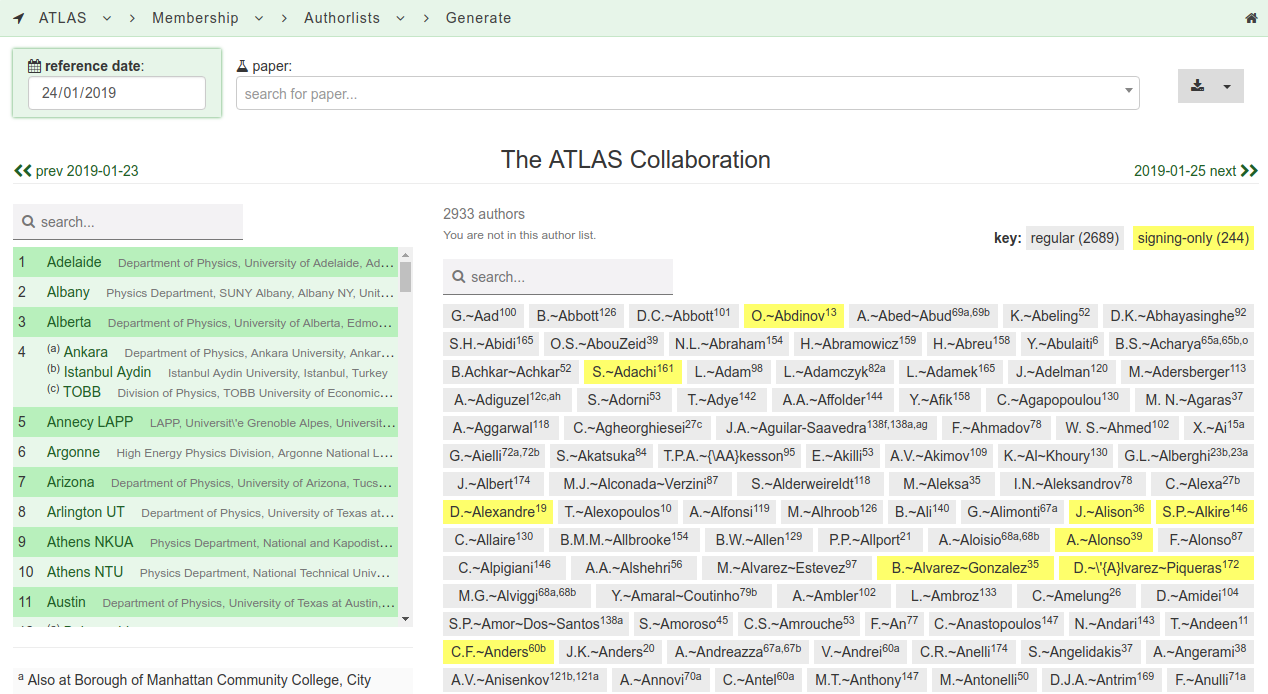
\includegraphics[width=0.9\textwidth]{authorlist_generate.png}
  \caption{Screenshot of Fence Authorlist generation interface.}
  \label{fig:po-ana-tree}
\end{figure}

\subsection{Fence Acknowledgement interfaces main functionalities (Gitlab, AFS ...)}

The creation of a new acknowledgement files with its relative push or save into CERN servers are made on the same way as the authorlists ones, during the process of the paper’s creation on Phase 1. The PO-members can create a new acknowledgment file and store it on its relative path or repository.
As for the authorlists we have an interface to resume all the acknowledgments created for each paper:
\centerline{<link here>}
From this list we have the entire list of papers which have an acknowledgment created using Fence system and allow users to download each version into different formats: .tex (the one used on the papers submission), .pdf and .docx. The icon on the download column distinguish the path of the file: it should be on a GitLab repository or store into internal CERN servers.

\centerline{<screenshot here>}

\subsection{Gitlab structure to organize ANA groups and repos}

ANA groups and repos are created in GitLab under the atlas-physics-office group. A different subgroup is created for every publication group, such as TOPQ, HIGG, PERF… where projects are referred with the prefix ANA- followed by the ref code of the publication. When a Phase 0 entry is created through Glance, the first internal note repository can be found in the project. Eventually a Paper, Pub-note or Conf-note repository will be added whenever the process reaches Phase 1. 

\subsection{Fence Gitlab class (middleware) to interact with Gitlab API}

As for all the other tools created under the Fence framework, many classes has been developed using oriented object programming, to provide the developers tools for a correct interaction between Fence and GitLab. Through the GitLab main class it’s possible to handle all the basic operations offered by GitLab itself: create, get and customize settings for projects, groups, branches…,  handle commits adding files and commit messages, and so on.
For every element in GitLab a resource class in Fence matches the specific role, so among all the classes at support for the main GitLab class we find the Branch, File and Commit classes, and Project, Group, Label and Member classes. 
